\documentclass[12pt]{article}
\usepackage[utf8]{inputenc}
\usepackage{natbib}
\usepackage{url}
\usepackage{graphicx}
\title{Mini Research Note on Animal Movement Modelling Tools}
\author{Simon Schiebel}
\date{\today}

\begin{document}

\maketitle

With increasing access to telemetry data of animal movement many new methods to further investigate them are developed (see \cite{florko_introduction_2025, butts_data-driven_2022, wang_derivations_2024, rieber_treed_2024}). Of special interest are open-source tools such as the R packages \textit{amt} \citep{signer_animal_2019} and \textit{moveHMM} \citep{michelot_movehmm_2016} which make complicated statistical methods easily usable for a wide audience. Even in an easy digestible way like that many of these functions are still not easy to comprehend (see Fig. \ref{fig:reading_doc}), but thankfully the authors of such packages are aware of that and also offer some very helpful guides such as \cite{fieberg_how_2021}. 

\begin{figure}
    \centering
    \includegraphics[width=0.5\linewidth]{figures/figure.pdf}
    \caption{Visualization of the process while researching a well documented but very confusing R package.}
    \label{fig:reading_doc}
\end{figure}

\bibliographystyle{plainnat}
\bibliography{bibliography/references.bib}
\end{document}